\documentclass[10pt,a4paper]{article}

% ATS-friendly, selectable text. Compile with pdfLaTeX, XeLaTeX, or LuaLaTeX.
\usepackage[utf8]{inputenc}
\usepackage[T1]{fontenc}
\usepackage{lmodern}
\usepackage[a4paper,top=1.0cm,bottom=0.95cm,left=1.35cm,right=1.35cm]{geometry}
\usepackage{graphicx}
\usepackage{xcolor}
\usepackage{enumitem}
\usepackage[hidelinks]{hyperref}
\usepackage{microtype}

\definecolor{ink}{HTML}{111111}
\definecolor{muted}{HTML}{444444}
\hypersetup{colorlinks=true,urlcolor=ink,linkcolor=ink}
\pagestyle{empty}
\setlength{\parindent}{0pt}
\setlength{\parskip}{0pt}
\setlist[itemize]{leftmargin=1.15em,itemsep=1pt,topsep=2pt,parsep=0pt}

\newcommand{\sectiontitle}[1]{%
  \vspace{7pt}\noindent\textbf{\large\MakeUppercase{#1}}\par
  \vspace{2pt}\hrule height 0.45pt\vspace{4pt}}
\newcommand{\entry}[3]{%
  \noindent\textbf{#1}\hfill\textbf{#2}\par
  \textit{#3}\par}
\newcommand{\project}[2]{%
  \noindent\textbf{#1}\hfill\textbf{#2}\par}
\newcommand{\tightitem}[1]{\item\small #1}

\begin{document}

% The portrait is deliberately kept rectangular and separate from the text flow.
\begin{minipage}[t]{0.77\textwidth}
  {\fontsize{25}{28}\selectfont\textbf{Salma IHSSAN}}\\[3pt]
  {\normalsize École Centrale de Lyon — Promotion 2027}\\
  {\normalsize Intelligence artificielle & génie logiciel}\\
  {\normalsize Stage PFE de 6 mois dès avril 2027}\\
  {\normalsize Lyon, France — Mobilité : France}\\[7pt]
  {\small
    \textbf{Tél. :} +33 7 45 20 74 18\quad
    \textbf{Email :} \href{mailto:salma.ihssan.pro@gmail.com}{salma.ihssan.pro@gmail.com}\\[2pt]
    \textbf{LinkedIn :} \href{https://linkedin.com/in/ihssan-salma}{linkedin.com/in/ihssan-salma}\quad
    \textbf{GitHub :} \href{https://github.com/Ihssan-Salma}{github.com/Ihssan-Salma}\\[2pt]
    \textbf{Portfolio :} \href{https://ihssan-salma.github.io/portfolio/}{ihssan-salma.github.io/portfolio/}
  }
\end{minipage}\hfill
\begin{minipage}[t]{0.19\textwidth}
  \centering
  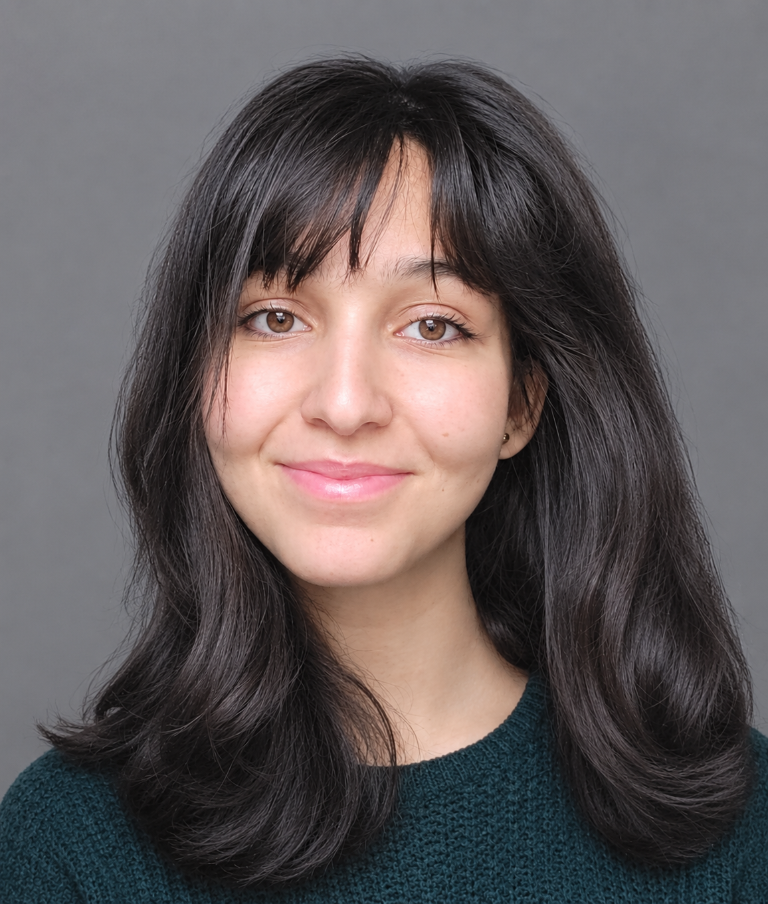
\includegraphics[width=3.05cm,height=3.60cm,keepaspectratio=true]{assets/salma-ihssan-portrait.png}
\end{minipage}

\sectiontitle{Profil}
Élève-ingénieure en double cursus ENSAM Meknès–Centrale Lyon et en Master 2 IA. Expérience en traitement de réclamations bancaires par LLM, RAG et orchestration d’agents. Je souhaite contribuer à des projets d’IA agentique et d’automatisation, en m’appuyant sur mes compétences en génie logiciel.

\sectiontitle{Formation}
\entry{École Centrale de Lyon — France}{2026–2027}{3e année du cycle ingénieur, option Informatique ; Master 2 Intelligence Artificielle.}
\vspace{3pt}
\entry{ENSAM Meknès — Maroc}{2022–2026}{Cycle ingénieur : génie logiciel et systèmes intelligents (2024–2026). Classes préparatoires intégrées (2022–2024).}

\sectiontitle{Expériences professionnelles}
\entry{Stagiaire ingénieure IA & Data — Attijariwafa bank}{Été 2026}{Casablanca, Maroc}
\begin{itemize}
  \tightitem{Conception d’un système de traitement des réclamations bancaires avec Llama 3, LangGraph, RAG et MCP : extraction d’informations, analyse de l’insatisfaction et de la sensibilité, priorisation et alertes urgentes.}
  \tightitem{Détection et masquage des données personnelles (PII) pour sécuriser le traitement.}
\end{itemize}
\vspace{2pt}
\entry{Stagiaire Data Analyst — Autoroutes du Maroc}{Été 2025}{Rabat, Maroc}
\begin{itemize}
  \tightitem{Analyse du trafic 2022–2024 : modèle en étoile, mesures DAX et tableaux de bord Power BI pour identifier les tendances de congestion.}
\end{itemize}

\sectiontitle{Projets sélectionnés}
\project{ReSlot AI — remplacement des réservations annulées}{2026 — en cours}
Architecture prévue à quatre agents : vérifier les créneaux, sélectionner les clients en attente, notifier et suivre les réponses. Intégration de Gmail, Calendar et Sheets avec isolation des données par entreprise.\\
\textit{Stack :} Python, FastAPI, MCP, PostgreSQL, Docker ; orchestration LangGraph en cours.
\vspace{4pt}

\project{Reconnaissance des émotions faciales}{2026}
Classification de sept expressions sur FER2013 par CNN : augmentation de données, équilibrage des classes et évaluation par F1 et matrice de confusion. Démonstration vidéo avec suivi des visages et lissage des prédictions.\\
\textit{Stack :} TensorFlow/Keras, OpenCV, CNN.
\vspace{4pt}

\project{eGrading — plateforme d’évaluation académique}{2025}
Espaces administrateur, enseignant et étudiant : publication des travaux, dépôt des réponses, correction et consultation des retours. API REST et interface web.\\
\textit{Stack :} Spring Boot, React/TypeScript, MySQL, MongoDB.
\vspace{4pt}

\project{Agile Tracker — gestion de projets en microservices}{Projet académique}
Backend de gestion des équipes, backlogs, sprints, tâches et temps ; bases séparées par domaine et services conteneurisés.\\
\textit{Stack :} Java 17, Spring Boot/JPA, PostgreSQL, Docker Compose.

\sectiontitle{Compétences techniques}
\textbf{IA & data :} Python, LLM, LangChain, LangGraph, LangSmith, RAG, MCP, PyTorch, TensorFlow, OpenCV, Pandas, NumPy, scikit-learn, Power BI.\\
\textbf{Développement :} Java, JavaScript, C++, SQL, NoSQL, FastAPI, React.\\
\textbf{Outils & méthodes :} Docker, Git, Linux, Prometheus, Grafana, Kubernetes (notions), Agile, Scrum, Jira.

\sectiontitle{Certifications & langues}
Linux Essentials — LPI ; Agents Fundamentals — Hugging Face.\\
Designing Agentic Systems with LangChain ; Multi-Agent Systems with LangGraph — DataCamp.\\
Introduction to Model Context Protocol — Claude Academy.\\
\textbf{Langues :} Français B2 ; Anglais B2 ; Arabe : langue maternelle.

\sectiontitle{Engagements & ouverture}
\textbf{Groupama / Centrale Lyon (2026) :} étude prospective des besoins agricoles à l’horizon 2040, proposition de valeur, modèle économique et pitch collectif.\\
\textbf{Hackathons :} Aidant 2026 (Sopra Steria, Crédit Agricole) ; Ramadan IA 2026.\\
\textbf{Vie associative :} membre active de Gadz’IT et du club social de l’ENSAM.

\end{document}
